% COVID-19-related disruptions in health services and data
% (c) 2023 Malcolm Gillies <malcolm.gillies@unsw.edu.au>
% https://github.com/mbg-unsw/pandemic-data-disruption
%
% This work is licensed under a
% Creative Commons Attribution-NonCommercial-ShareAlike 4.0
% International Licence
\documentclass[aspectratio=169,12pt]{beamer} % XXXX fix AR here
\usepackage{pgfpages}
\usepackage{fancyvrb}
\usepackage{pgfplots}
%\usepackage[latin1]{inputenc}
%\usepackage[T1]{fontenc}
%\usepackage{textcomp}
%\usefonttheme{serif} % need this with Charter font
\usetheme{auriga}  % using default now
\usecolortheme{auriga}  % using default now
%\usepackage[libertine]{libertine} % not using osf (old-style figures)
%\usepackage[scale=0.9]{tgheros} % scale to match libertine
%\usepackage[varqu,varl]{inconsolata}
%\usepackage[libertine]{newtxmath}
\usepackage{graphicx}
\usepackage{tikz}
\usetikzlibrary{shadows}
\usepackage{tikzpagenodes}
\usepackage{natbib}
\usepackage{gitinfo2}

\pgfplotsset{compat=1.17}
\hypersetup{pdfencoding=auto}

\renewcommand{\gitMark}{\color{lightgray}\texttt{\tiny\gitBranch\,@\,\gitAbbrevHash\,\gitAuthorDate}}

%\renewcommand{\bibsection}{} % suppress "References" section

%\setbeamertemplate{navigation symbols}{} % remove navigation symbols
%\setbeamercolor*{item}{fg=darkred}

\title{COVID-19-related disruptions in\\health services and data:\\Tracing causes and effects}
\author{Malcolm Gillies <malcolm.gillies@unsw.edu.au>}
\institute{27 April 2023}
\usebackgroundtemplate{%

\includegraphics[width=\paperwidth]{ref/micre-blank.PNG}
\begin{tikzpicture}[remember picture,overlay]
    \node[anchor=south east,scale=1,rotate=90] at ([shift={(0cm,0cm)}]current page marginpar area.north east) {\gitMark};
\end{tikzpicture}%
}


\newif\ifsidebartheme
\sidebarthemefalse

\newdimen\contentheight
\newdimen\contentwidth
\newdimen\contentleft
\newdimen\contentbottom
\makeatletter
\newcommand*{\calculatespace}{%
    \contentheight=\paperheight%
    \ifx\beamer@frametitle\@empty%
        \setbox\@tempboxa=\box\voidb@x%
      \else%
        \setbox\@tempboxa=\vbox{%
          \vbox{}%
          {\parskip0pt\usebeamertemplate***{frametitle}}%
        }%
        \ifsidebartheme%
          \advance\contentheight by-1em%
        \fi%
      \fi%
    \advance\contentheight by-\ht\@tempboxa%
    \advance\contentheight by-\dp\@tempboxa%
    \advance\contentheight by-\beamer@frametopskip%
    \ifbeamer@plainframe%
    \contentbottom=0pt%
    \else%
    \advance\contentheight by-\headheight%
    \advance\contentheight by\headdp%
    \advance\contentheight by-\footheight%
    \advance\contentheight by4pt%
    \contentbottom=\footheight%
    \advance\contentbottom by-4pt%
    \fi%
    \contentwidth=\paperwidth%
    \ifbeamer@plainframe%
    \contentleft=0pt%
    \else%
    \advance\contentwidth by-\beamer@rightsidebar%
    \advance\contentwidth by-\beamer@leftsidebar\relax%
    \contentleft=\beamer@leftsidebar%
    \fi%
}
\makeatother

\begin{document}

\setbeamercolor{page number in head/foot}{fg=white}

{
\usebackgroundtemplate{
\includegraphics[width=\paperwidth]{ref/micre.PNG}}
\setbeamercolor{title page}{fg=white}
  \begin{frame}[plain]
    \titlepage
  \end{frame}
}

{
\usebackgroundtemplate{%

\includegraphics[width=\paperwidth]{ref/micre-partners.pdf}}
\begin{frame}{}
\end{frame}
}

\begin{frame}{Outline}
	\begin{itemize}
		\item Changes in antibiotic use in 2020
		\item Changes in antidepressant use in 2020
		\item \emph{Why the changes?}
		\item \emph{What happened exactly?}
		\item \emph{How should we design future studies?}
	\end{itemize}
\end{frame}

\begin{frame}{Study 1: PBS antibiotics in 2020}
\centering
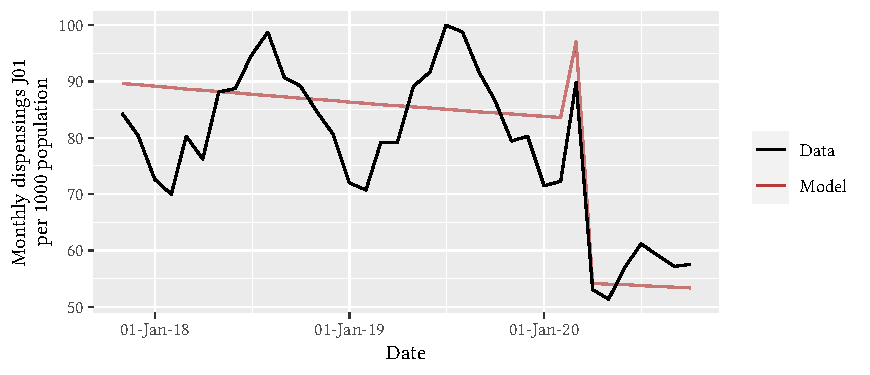
\includegraphics{ref/latex-j01armap3-1.pdf}
\end{frame}

\begin{frame}{Human behaviour c. March 2020}
\centering
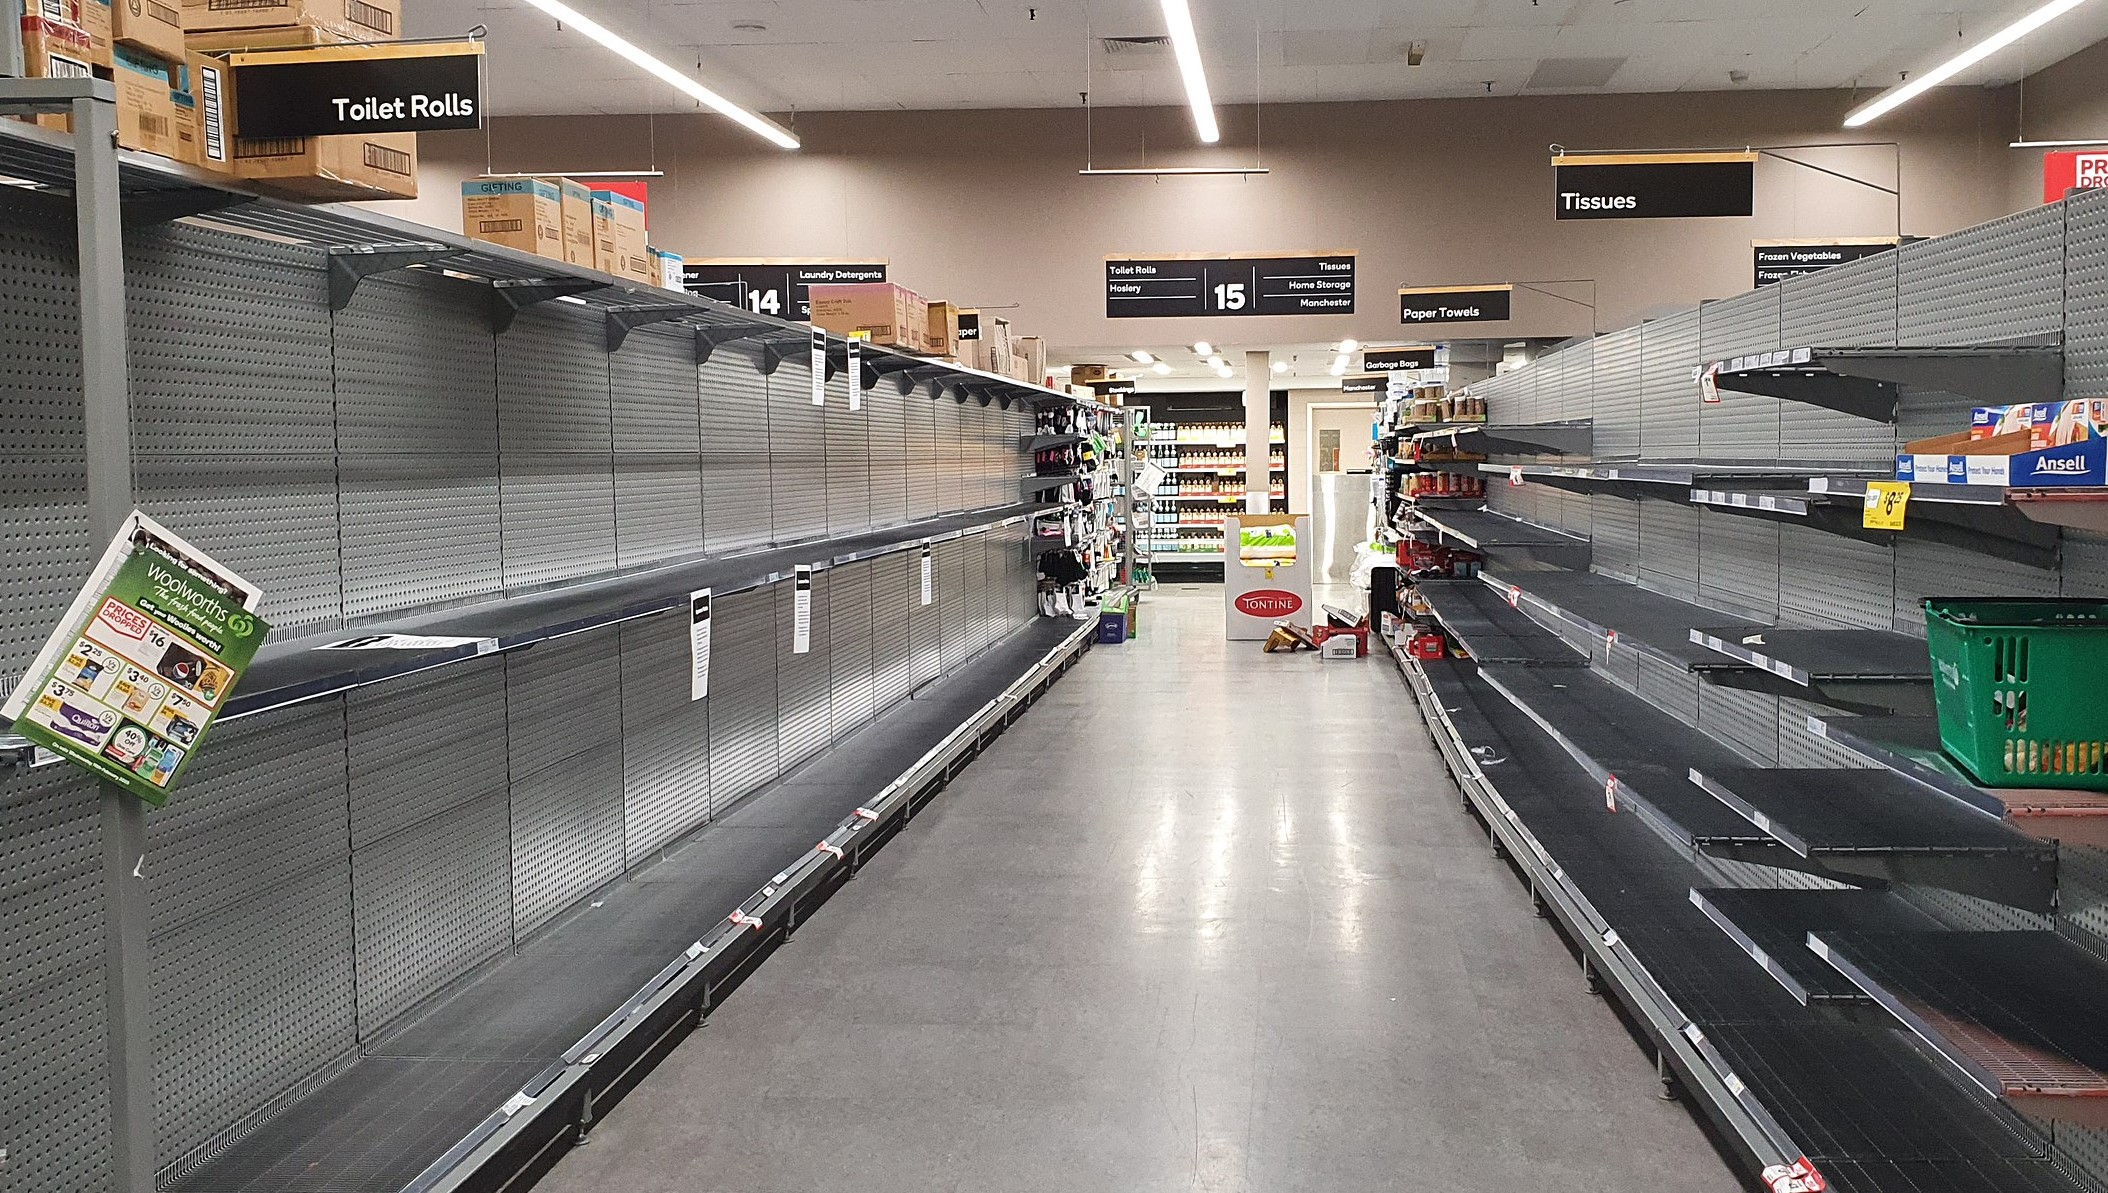
\includegraphics[height=0.75\textheight]
	{ref/toilet-paper-crop.jpg}

	\tiny 9 March 2020

	\copyright\: Christopher Corneschi.
	Reproduced under CC-BY-SA licence [cropped from original]
	% XXXX nice to rotate this and put on the right
\end{frame}

\begin{frame}{Google mobility data, Sydney, 2020}
\centering
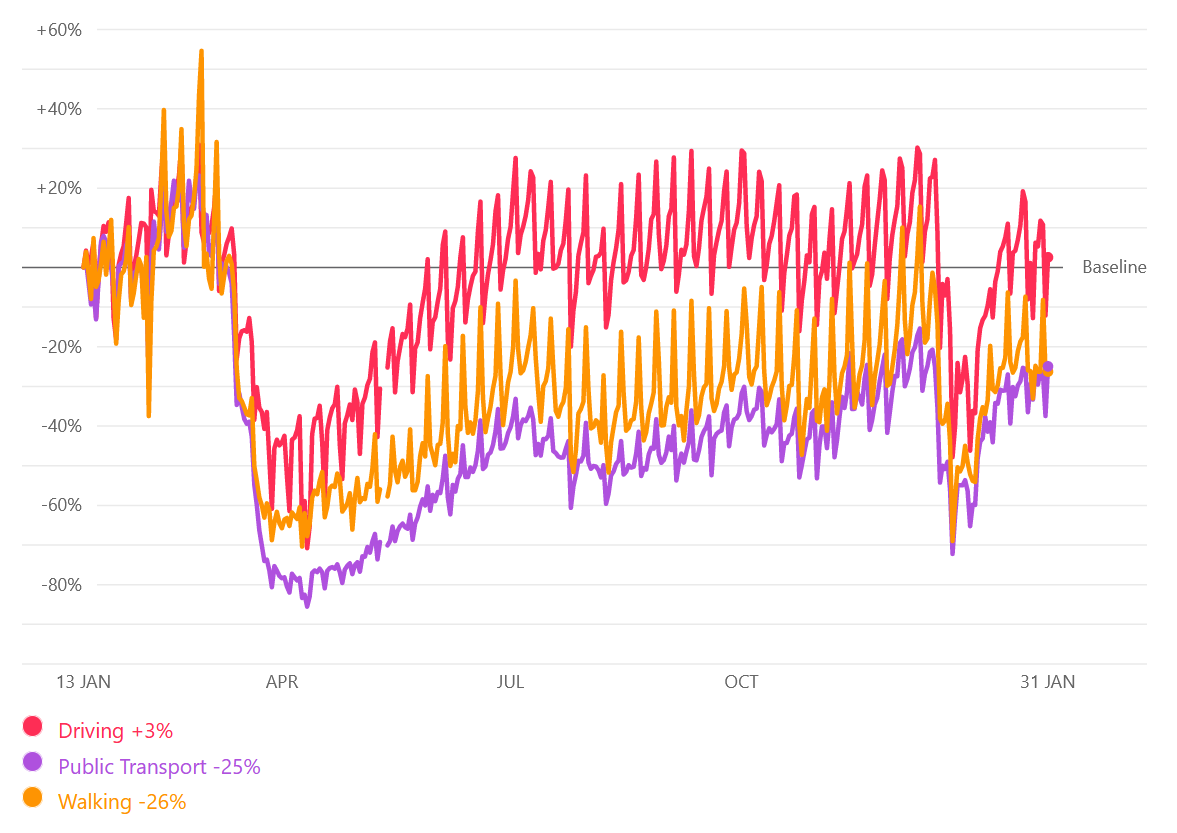
\includegraphics[height=0.8\textheight]
        {ref/google-mobility-20210202.PNG}
% https://covid19.apple.com/mobility
\end{frame}

\begin{frame}{Top 10 antibiotics step changes}
\centering
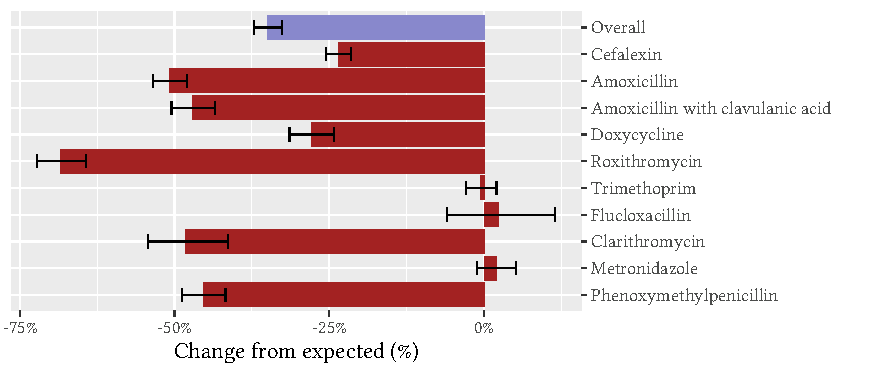
\includegraphics{ref/latex-j01arimatab-1.pdf}
\end{frame}

\begin{frame}{Changes in primary care consultation rates}
\centering
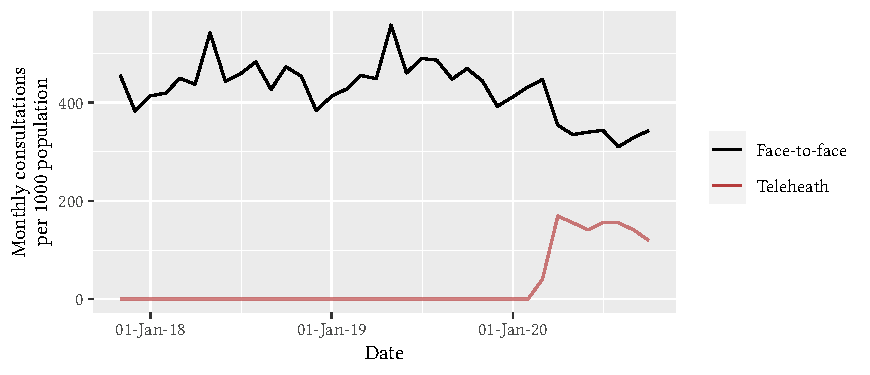
\includegraphics{ref/latex-suppmbs-1.pdf}
\nocite{gillies_2022}
\end{frame}

\begin{frame}{Antibiotic changes by prescriber specialty}
\centering
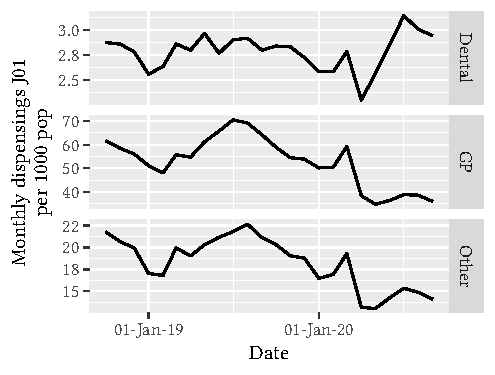
\includegraphics{ref/latex-j01specialty-1.pdf}
\end{frame}

\begin{frame}{What came first?}
\centering
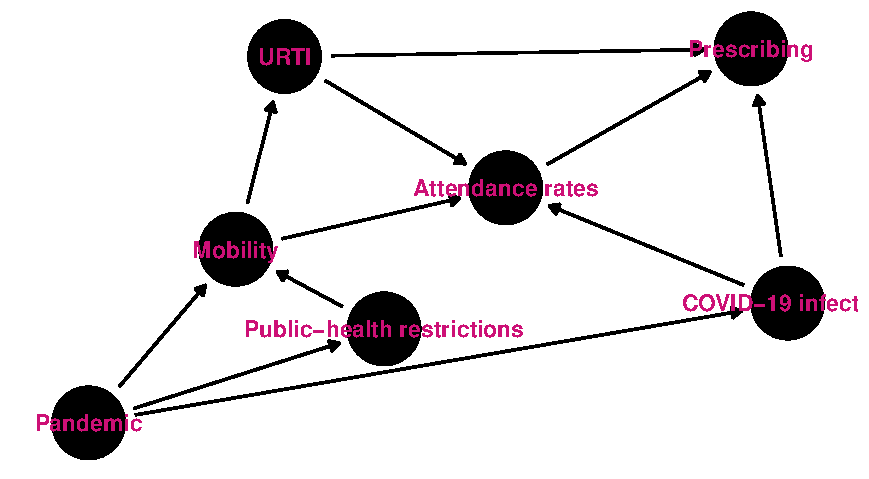
\includegraphics[height=0.8\textheight]
        {ref/dag.pdf}
\end{frame}

\begin{frame}{Study 2: PBS antidepressants in 2020}
\centering
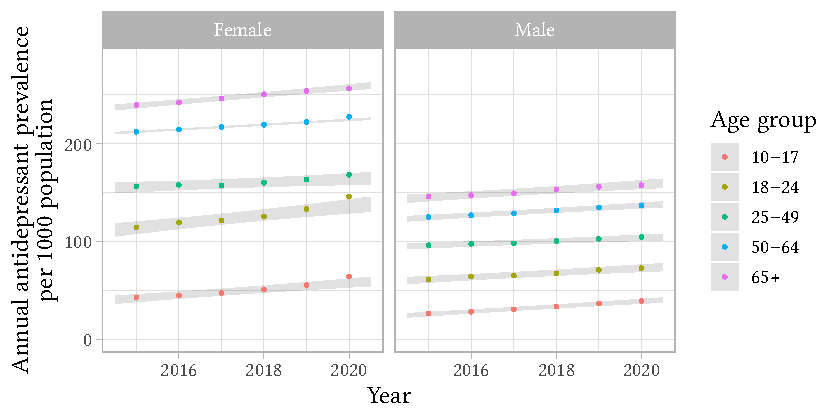
\includegraphics[height=0.8\textheight]
        {ref/covid19mh-prev-age.pdf}
	\nocite{costa_2023}
\end{frame}

\begin{frame}{ABS Estimated Resident Population: Projected vs Reported 1}
	\center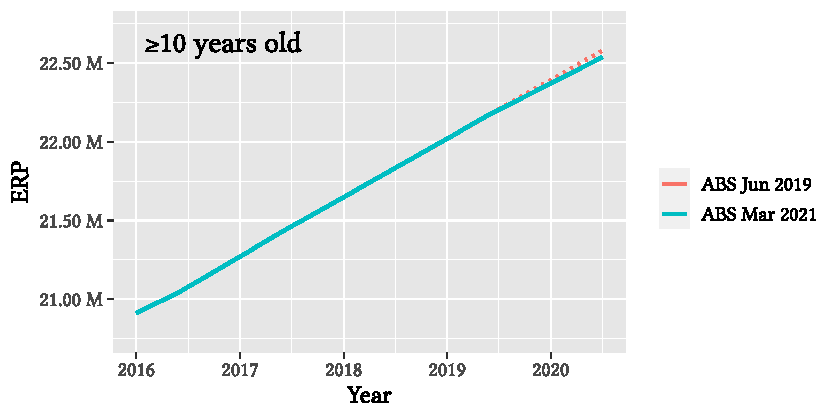
\includegraphics[height=0.75\textheight]{ref/pops-overall.pdf}
	\begin{flushright}\tiny\texttt{\url{https://www.abs.gov.au/statistics/people/population/national-state-and-territory-population}}\end{flushright}
\end{frame}

\begin{frame}{ABS Estimated Resident Population: Projected vs Reported 2}
	\center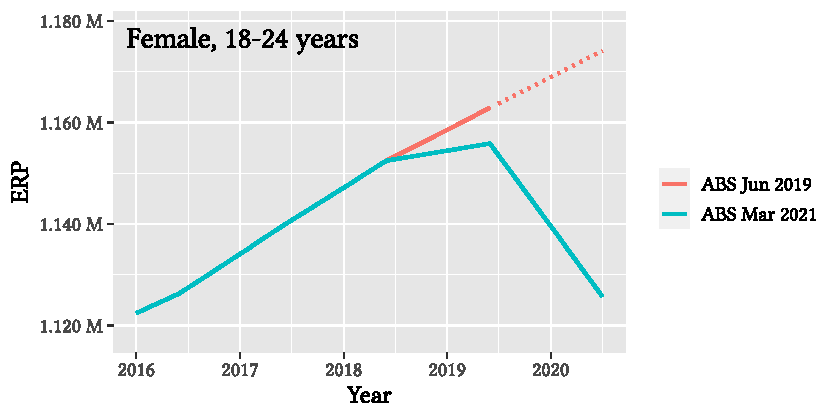
\includegraphics[height=0.75\textheight]{ref/pops-f18-24.pdf}
	\begin{flushright}\tiny\texttt{\url{https://www.abs.gov.au/statistics/people/population/national-state-and-territory-population}}\end{flushright}
\end{frame}

\begin{frame}{ABS components of population growth}

	\center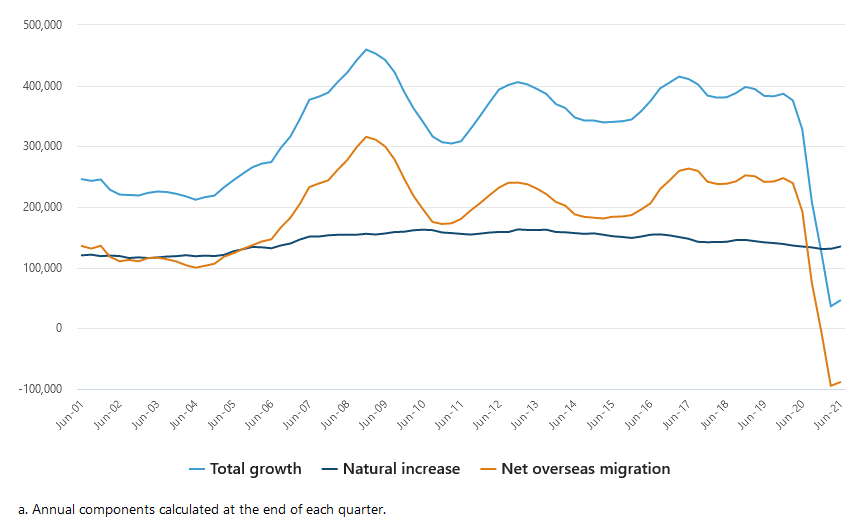
\includegraphics[height=0.75\textheight]{ref/pop-components.PNG}
	\begin{flushright}\tiny\texttt{\url{https://www.abs.gov.au/statistics/people/population/national-state-and-territory-population}}\end{flushright}
\end{frame}

\begin{frame}{Net overseas migration: PBS/MBS eligibility?}
	\center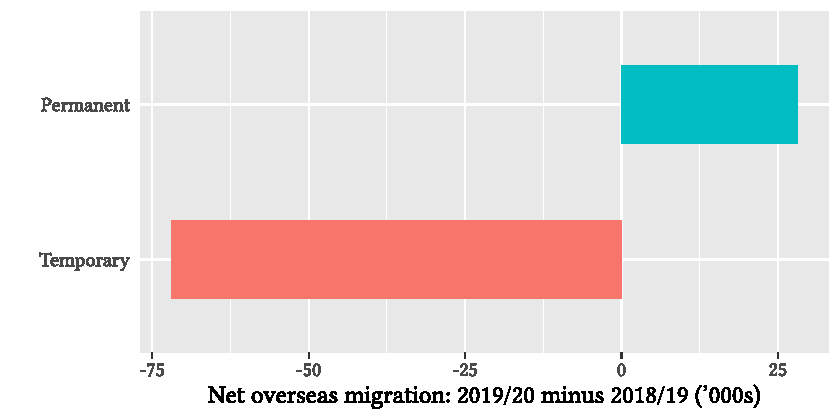
\includegraphics[height=0.75\textheight]{ref/pops-nom.pdf}
	\begin{flushright}\tiny\texttt{\url{https://www.abs.gov.au/statistics/people/population/migration-australia/latest-release}}\end{flushright}
\end{frame}

\begin{frame}{Some ideas about what to do}
\calculatespace%
\begin{columns}
\begin{column}{0.20\contentwidth}
\begin{tikzpicture}
  \node[drop shadow={shadow xshift=.8ex,shadow yshift=-.8ex},fill=white,draw] at (0,0) {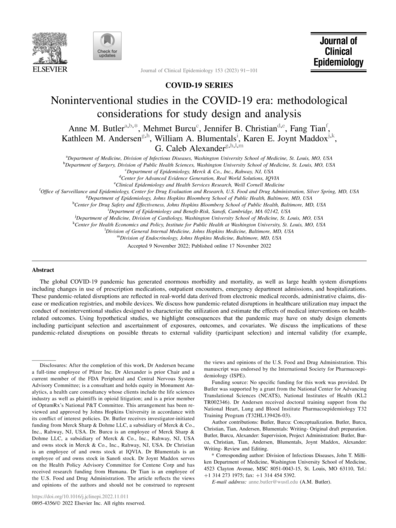
\includegraphics[width=\textwidth]{ref/butler_sm.png}};
\end{tikzpicture}
\end{column}
\begin{column}{0.70\contentwidth}
	\begin{itemize}
		\item A.~M. Butler, M.~Burcu, J.~B. Christian, F.~Tian,
		\emph{et al.} Noninterventional studies in the {COVID-19} era:
		methodological considerations for study design \& analysis. \\
		\emph{J Clin Epi}, 153:\penalty0 91--101, 2023.
\nocite{butler_2023}
	\end{itemize}
\end{column}
\end{columns}
\end{frame}

\begin{frame}{Study design elements to consider}
	\begin{itemize}
		\item Participant selection
		\item Exposure assessment
		\item Outcome assessment
		\item Covariate assessment
		\item Competing risks
	\end{itemize}
\end{frame}

\begin{frame}{Approaches to characterise or mitigate bias}
\calculatespace%
\begin{columns}
\begin{column}{0.45\contentwidth}
	\begin{itemize}
		\item Assess confounder time trends
		\item Consider missing data strategies
		\item Use negative controls
		\item Consider COVID-19 infection Hx
		\item Censor on COVID-19 diagnosis
		\item Adjust for COVID-19 status
	\end{itemize}
\end{column}
\begin{column}{0.45\contentwidth}
	\begin{itemize}
		\item Account for calendar time
		\item Account for factors with differential COVID-19 impact
		\item Do sensitivity analyses
		\item Replicate with different data sources
		\item Leverage additional data sources
	\end{itemize}
\end{column}
\end{columns}
\end{frame}

\begin{frame}{Our experience so far}
	\begin{itemize}
		\item Interrupted time series analyses
		\item Simple approaches like deleting or aggregating
		\item TODO: Dealing with ``phases'' of the pandemic
		\item TODO: revisit denominator data
	\end{itemize}
\end{frame}

\begin{frame}{Summary}
	\begin{itemize}
		\item Think about causal mechanisms carefully
		\item Consider aggregate and disaggregate analyses
		\item Things are unpredictable and keep changing
		\item We need to share good practices
	\end{itemize}
\end{frame}

\begin{frame}{Thanks}
    \begin{itemize}
        \item Australian Government Services Australia for providing the data
	\item My co-authors, especially Juliana, Andrea and Helga
	\item Melisa Litchfield for assisting with data access and ethics approval
	\item All the other Medicines Intelligence Research Program people at SPH
    \end{itemize}
\end{frame}

\begin{frame}{References}
%        \bibliographystyle{apalike}
%        \bibliographystyle{abbrv}
        \tiny\bibliography{pandemic-disruption.bib}
        \bibliographystyle{abbrvnat}
\end{frame}

\end{document}
